\chapter{Simulación de uso del sistema}
En los requisitos funcionales (Sección 7.2.1) se ha hecho una explicación de las diferentes acciones que se pueden realizar en el sistema, y en los capítulos 4 y 5 una explicación de como esas acciones funcionan a nivel de código. En este capítulo se muestra de forma visual como el sistema funciona con las acciones más comunes, es decir, con aquellas que un usuario va a realizar con más frecuencia. Estas acciones son:

\section{Introducir un producto en el frigorífico}
Al introducir un producto en el frigorífico, primero éste tiene que existir en el apartado de 'Productos'. Si el producto es uno que no precisa de tarjeta RFID, simplemente lo introducimos en el frigorífico y se actualiza la cantidad de ese producto automáticamente detectando el peso de éste. En la Figura \ref{fig:i1} podemos apreciar como había cero refrescos dentro del frigorífico, y en la Figura \ref{fig:i2} que al introducirlo ha detectado que la cantidad ha aumentado a un refresco.

\begin{figure}[h] 
    \centering
    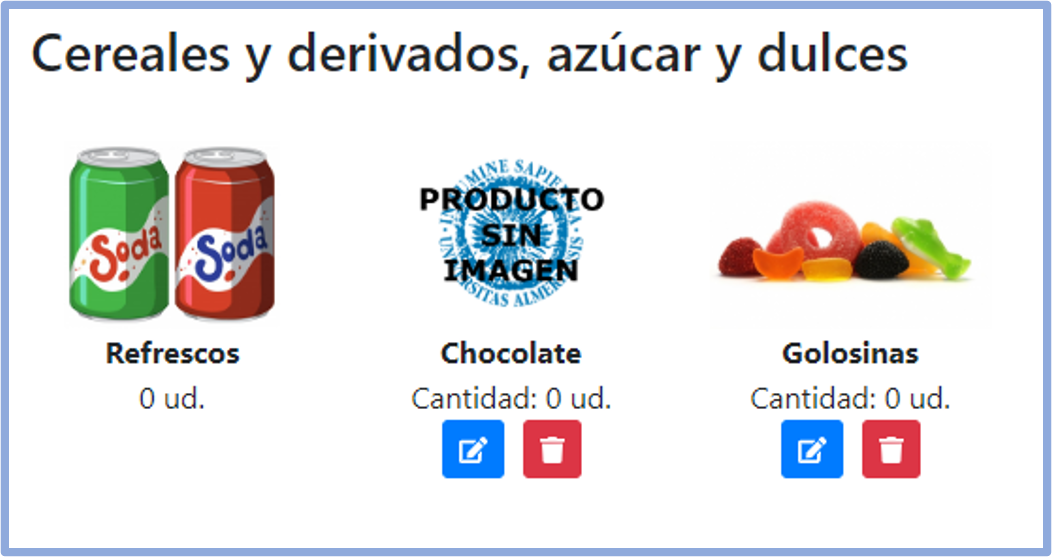
\includegraphics[width=.70\textwidth]{capitulos/capitulo10/introducir/1.png}
    \caption{Producto sin RFID sin introducir en el frigorífico.}
    \label{fig:i1}
\end{figure}

\begin{figure}[h] 
    \centering
    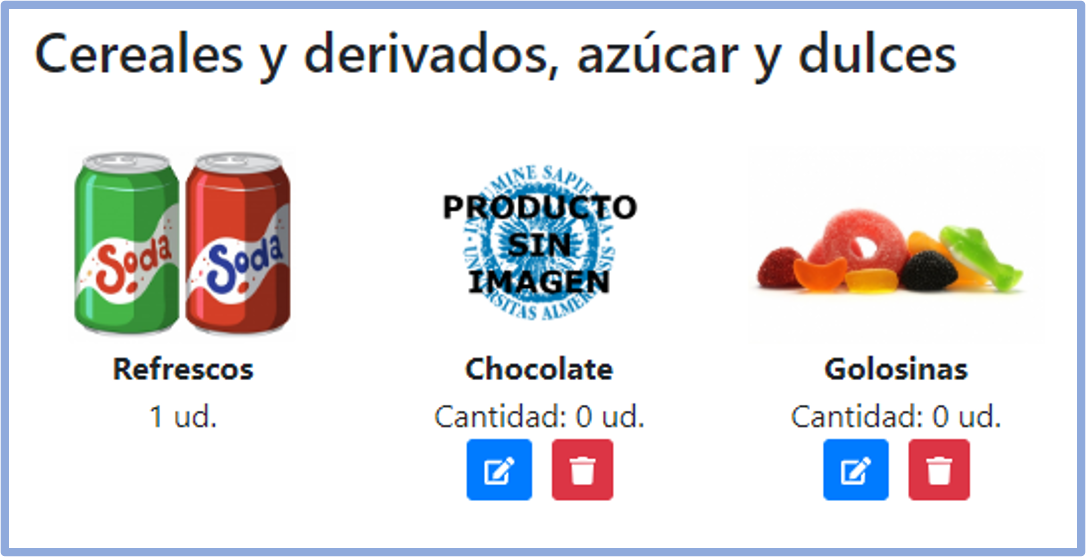
\includegraphics[width=.70\textwidth]{capitulos/capitulo10/introducir/2.png}
    \caption{Producto sin RFID introducido en el frigorífico.}
    \label{fig:i2}
\end{figure}

\newpage
Si el producto precisa de tarjeta RFID, debemos de añadirlo en el apartado de 'Etiquetas', junto con la cantidad que vamos a introducir de este producto (Figura \ref{fig:i4}). Podemos apreciar también en la Figura \ref{fig:i3} como la cantidad del producto antes de introducirlo es cero.

\begin{figure}[h] 
    \centering
    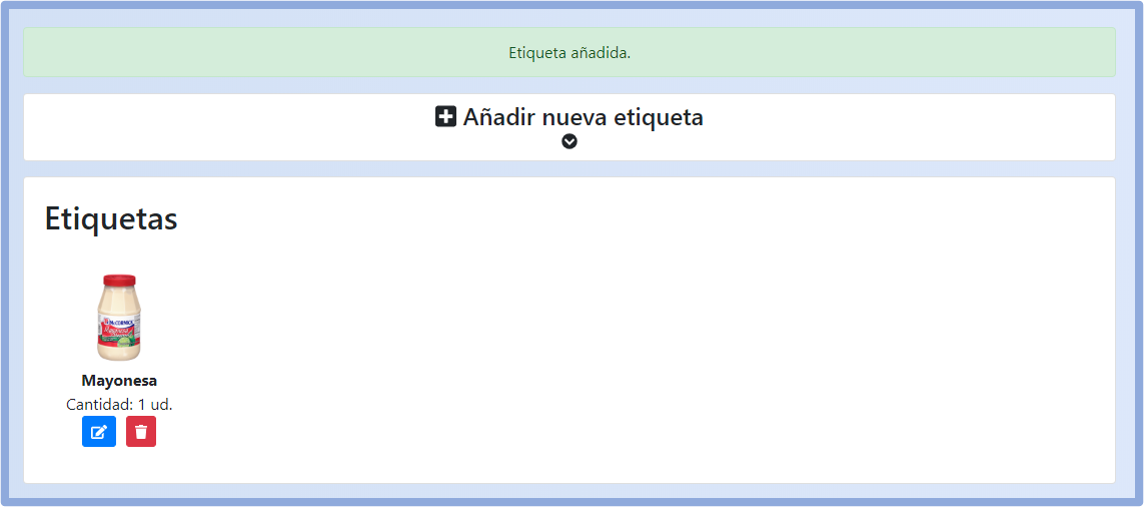
\includegraphics[width=.90\textwidth]{capitulos/capitulo10/introducir/4.png}
    \caption{Apartado 'Etiquetas' antes de introducir el producto.}
    \label{fig:i4}
\end{figure}

\begin{figure}[h] 
    \centering
    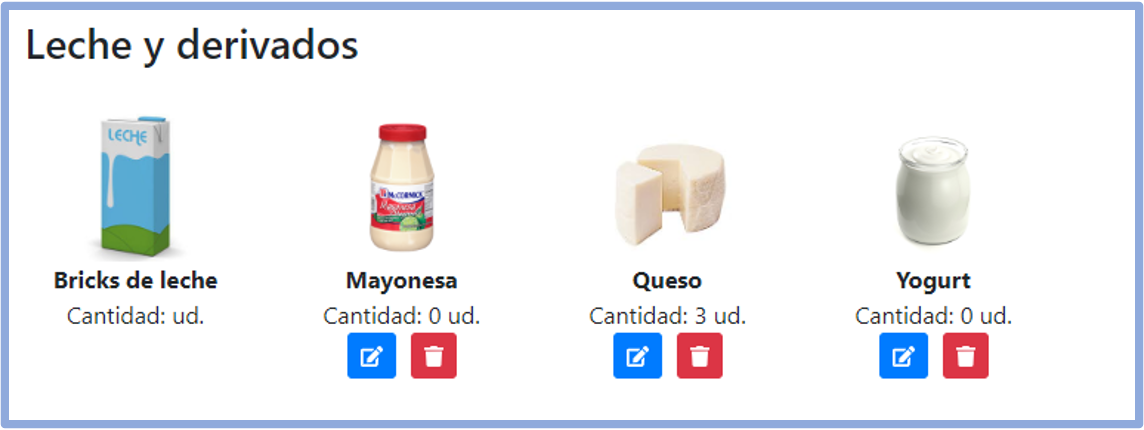
\includegraphics[width=.80\textwidth]{capitulos/capitulo10/introducir/3.png}
    \caption{Apartado 'Productos' antes de introducir el producto.}
    \label{fig:i3}
\end{figure}

\newpage
Una vez añadido, simplemente se debe de pasar el producto con la etiqueta RFID por el lector, y el sistema aplicará el producto como introducido, eliminando la tarjeta (Figura \ref{fig:i5}) e incrementando la cantidad del producto (Figura \ref{fig:i6}). También confirmará el proceso encendiendo un LED al lado del sensor RFID que especifica que se ha hecho todo el proceso correctamente.

\begin{figure}[h] 
    \centering
    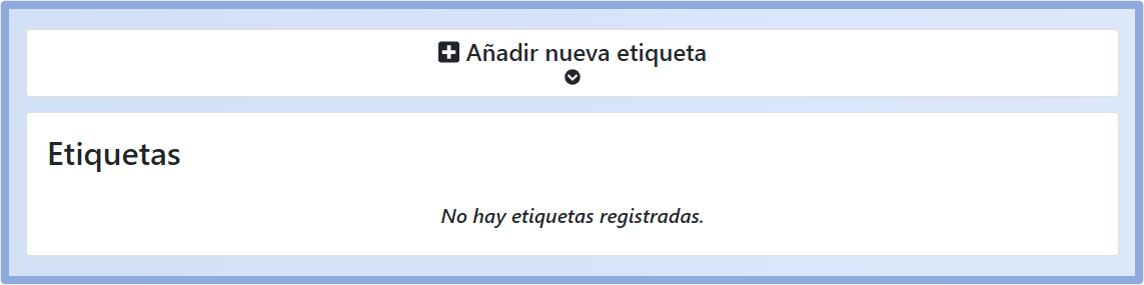
\includegraphics[width=.90\textwidth]{capitulos/capitulo10/introducir/5.png}
    \caption{Apartado 'Etiquetas' después de introducir el producto.}
    \label{fig:i5}
\end{figure}
\begin{figure}[h] 
    \centering
    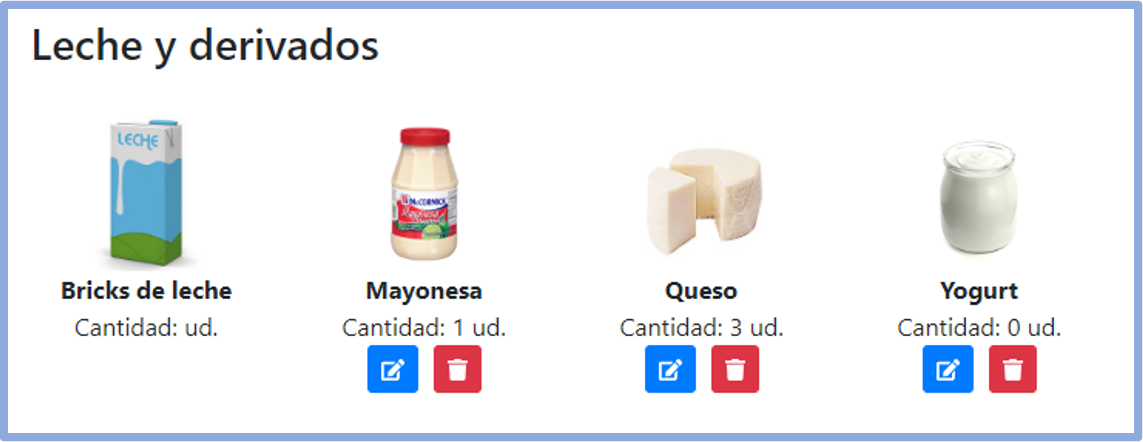
\includegraphics[width=.80\textwidth]{capitulos/capitulo10/introducir/6.png}
    \caption{Apartado 'Productos' después de introducir el producto.}
    \label{fig:i6}
\end{figure}

Se puede ver está acción de forma más visual en un vídeo en el siguiente enlace: \url{https://youtu.be/MGe1UsX1gB0}.

\section{Sacar un producto del frigorífico}
Al sacar el producto del frigorífico hay que distinguir entre dos tipos de productos. Si el producto es uno que no precisa de tarjeta RFID, simplemente se saca del frigorífico y se actualiza la cantidad de ese producto automáticamente detectando el peso de éste. En la Figura \ref{fig:s1} podemos apreciar como había un refrescos dentro del frigorífico, y en la Figura \ref{fig:s2} al sacarlo, ha detectado que la cantidad ha descendido a cero refrescos.

\begin{figure}[h] 
    \centering
    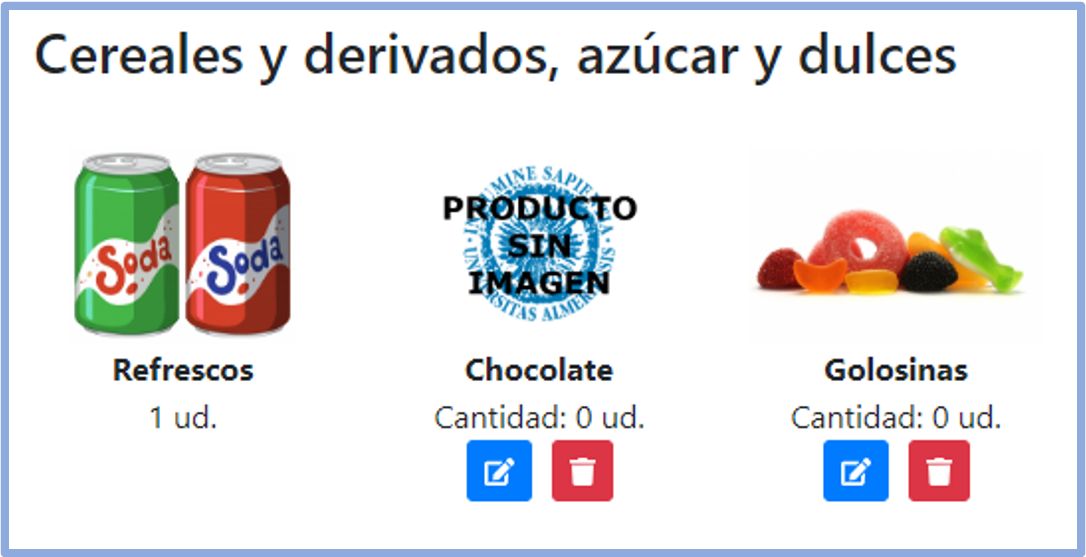
\includegraphics[width=.70\textwidth]{capitulos/capitulo10/sacar/1.png}
    \caption{Producto sin RFID sin sacar del frigorífico.}
    \label{fig:s1}
\end{figure}

\begin{figure}[h] 
    \centering
    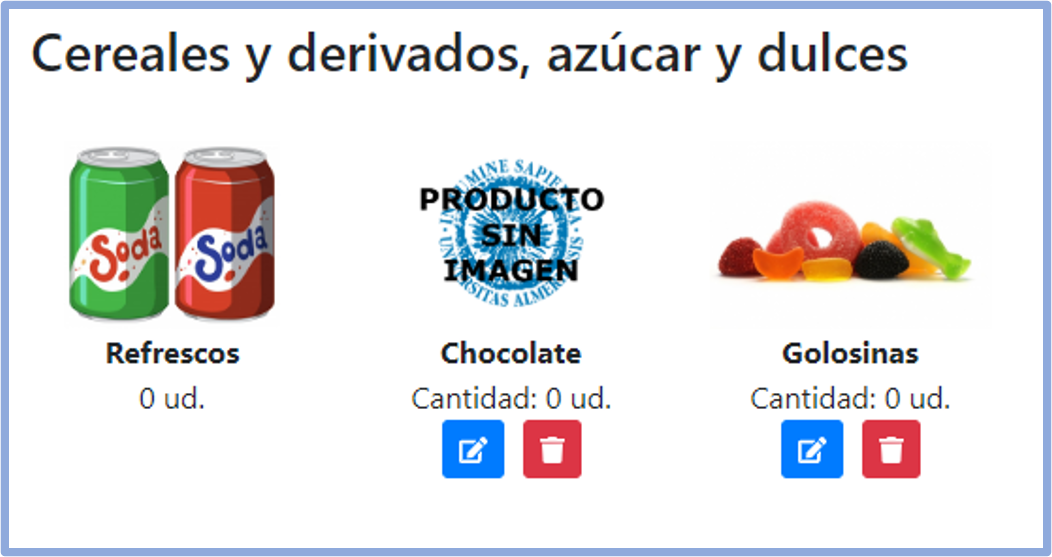
\includegraphics[width=.70\textwidth]{capitulos/capitulo10/sacar/2.png}
    \caption{Producto sin RFID sacado del frigorífico.}
    \label{fig:s2}
\end{figure}

Antes de sacar el producto, podemos apreciar que hay una unidad del producto 'Mayonesa' (Figura \ref{fig:s3}). Al sacarlo, simplemente se debe de pasar el producto con la etiqueta RFID por el lector, y el sistema aplicará el producto como sacado, decrementando la cantidad del producto (Figura \ref{fig:s4}). También confirmará el proceso encendiendo un LED al lado del sensor RFID que especifica que se ha hecho todo el proceso correctamente.

\begin{figure}[h] 
    \centering
    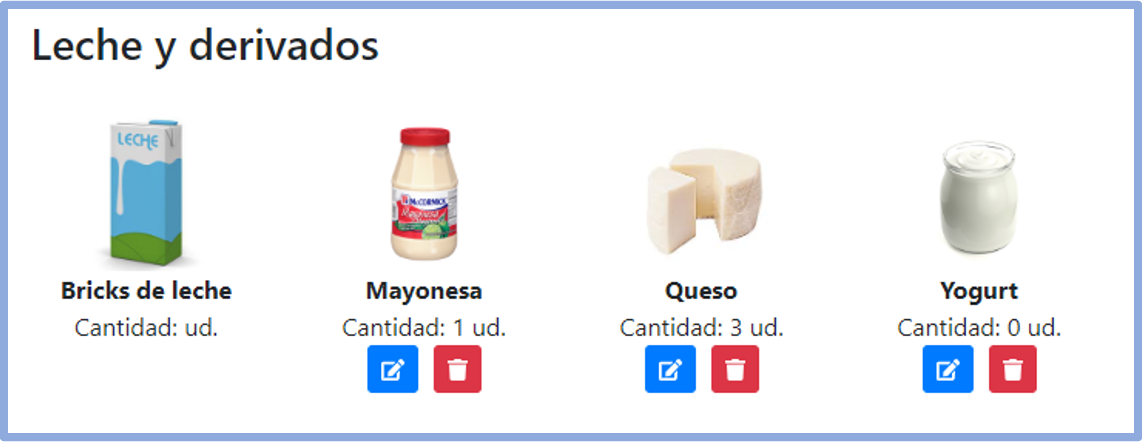
\includegraphics[width=.80\textwidth]{capitulos/capitulo10/sacar/3.png}
    \caption{Apartado 'Productos' antes de sacar el producto.}
    \label{fig:s3}
\end{figure}
\begin{figure}[h] 
    \centering
    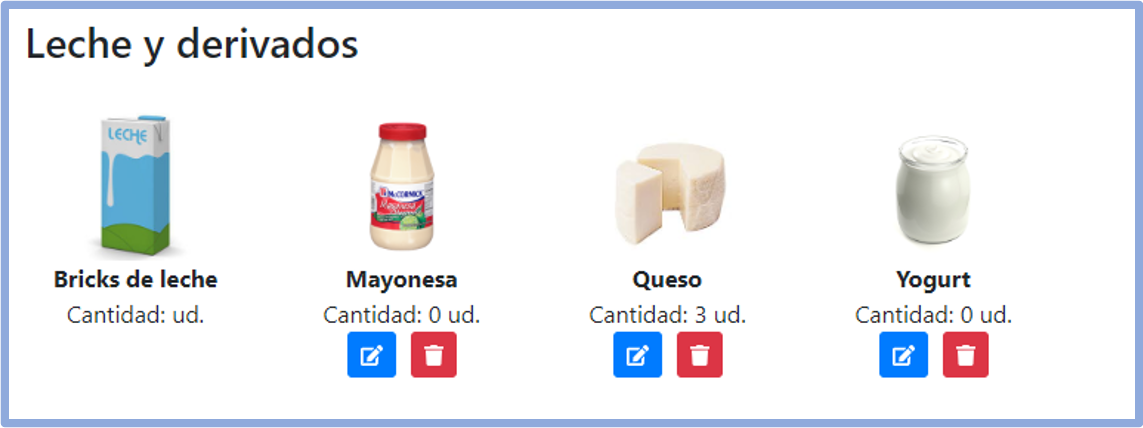
\includegraphics[width=.80\textwidth]{capitulos/capitulo10/sacar/4.png}
    \caption{Apartado 'Productos' después de sacar el producto.}
    \label{fig:s4}
\end{figure}

\newpage
Se puede ver está acción de forma más visual en un vídeo en el siguiente enlace: \url{https://youtu.be/k6kQK8lmE7E}.

\section{Lista de la compra}
El administrador puede cambiar los umbrales de cantidad de un producto para especificar cuando añadir un producto a la lista de la compra. En este ejemplo está configurado a 2 unidades. Como se puede ver en la Figura \ref{fig:l1}, hay 3 unidades de mayonesa, y en la Figura \ref{fig:l2} como no está añadido a la lista de la compra

\begin{figure}[h] 
    \centering
    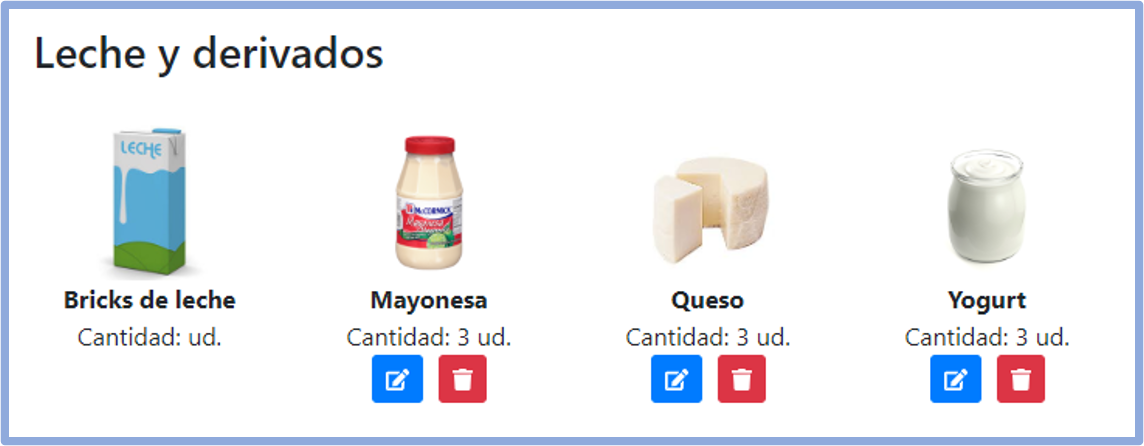
\includegraphics[width=.80\textwidth]{capitulos/capitulo10/listacompra/1.png}
    \caption{Producto antes de añadirse a la lista de la compra.}
    \label{fig:l1}
\end{figure}

\begin{figure}[h] 
    \centering
    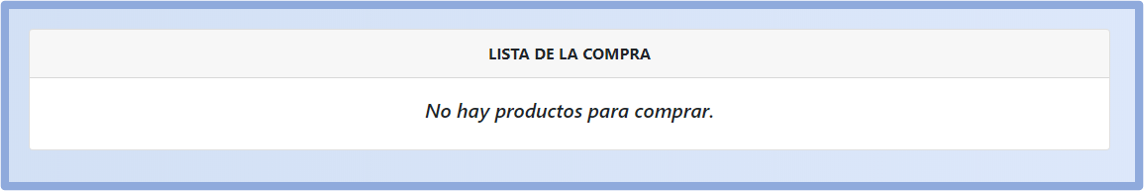
\includegraphics[width=.80\textwidth]{capitulos/capitulo10/listacompra/2.png}
    \caption{Lista de la compra vacía.}
    \label{fig:l2}
\end{figure}

\newpage
Si se sacan dos unidades de mayonesa, el producto estaría por debajo del umbral para añadir a la lista de la compra, concretamente con una unidad (Figura \ref{fig:l3}), por lo que el producto se añade automáticamente a la lista de la compra (Figura \ref{fig:l4}), además de enviar un mensaje por correo al usuario administrador (Figura \ref{fig:l5}). 

\begin{figure}[h] 
    \centering
    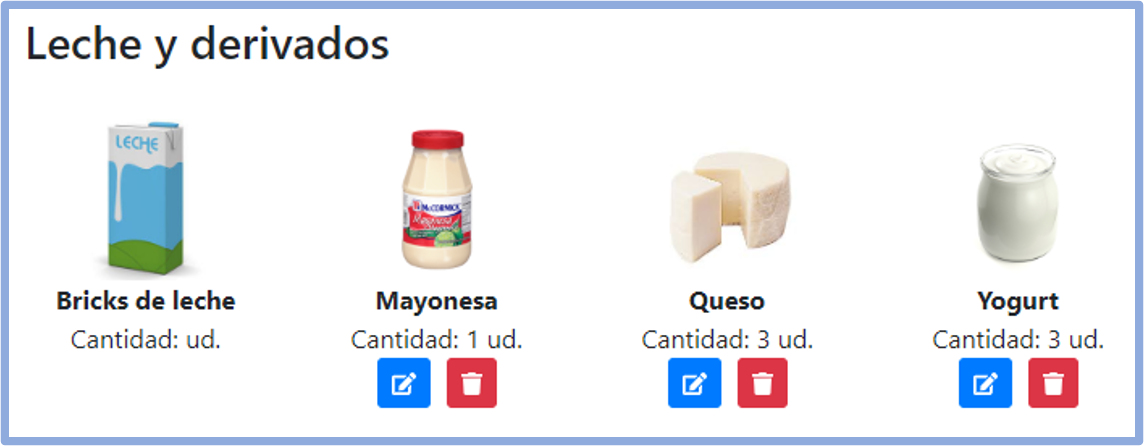
\includegraphics[width=.80\textwidth]{capitulos/capitulo10/listacompra/3.png}
    \caption{Producto después de añadirse a la lista de la compra.}
    \label{fig:l3}
\end{figure}

\begin{figure}[h] 
    \centering
    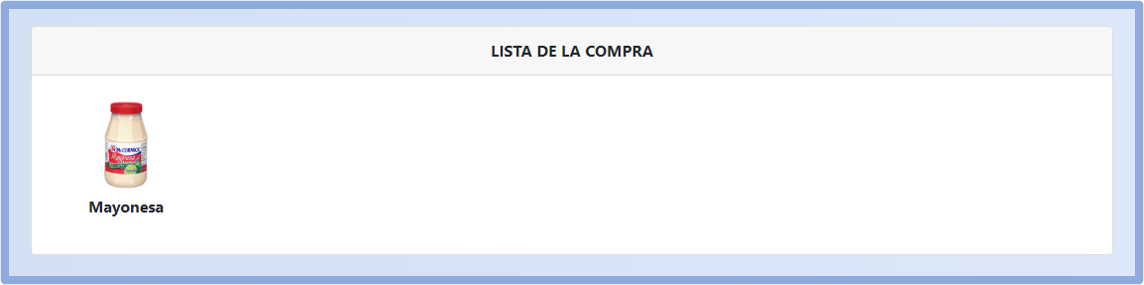
\includegraphics[width=.80\textwidth]{capitulos/capitulo10/listacompra/4.png}
    \caption{Lista de la compra con un producto.}
    \label{fig:l4}
\end{figure}

\begin{figure}[h] 
    \centering
    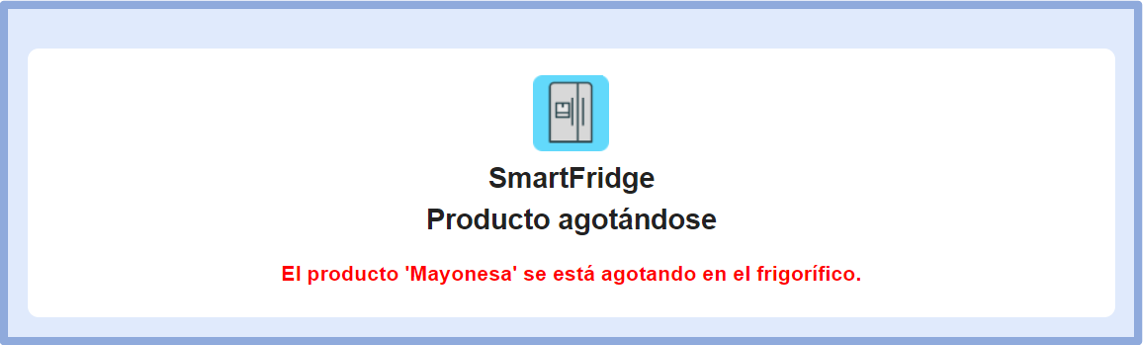
\includegraphics[width=.80\textwidth]{capitulos/capitulo10/listacompra/5.png}
    \caption{Mensaje avisando de producto agotado.}
    \label{fig:l5}
\end{figure}

\newpage
Se puede ver está acción de forma más visual en un vídeo en el siguiente enlace: \url{https://youtu.be/cL2yjecfi6Y}.

\section{Actividad}
Si un usuario está identificado mediante RFID y saca un producto del frigorífico, éste se reflejará en la interfaz, en el apartado de Actividad con su sesión iniciada.

Primeramente se puede ver en la Figura \ref{fig:a1} que no hay ninguna actividad en el día de hoy, a continuación, el usuario se identifica mediante RFID y saca un bote de mayonesa, y podemos ver como el sistema ha reflejado el producto y la hora en la que el usuario ha cogido el producto (Figura \ref{fig:a2}).

\begin{figure}[h] 
    \centering
    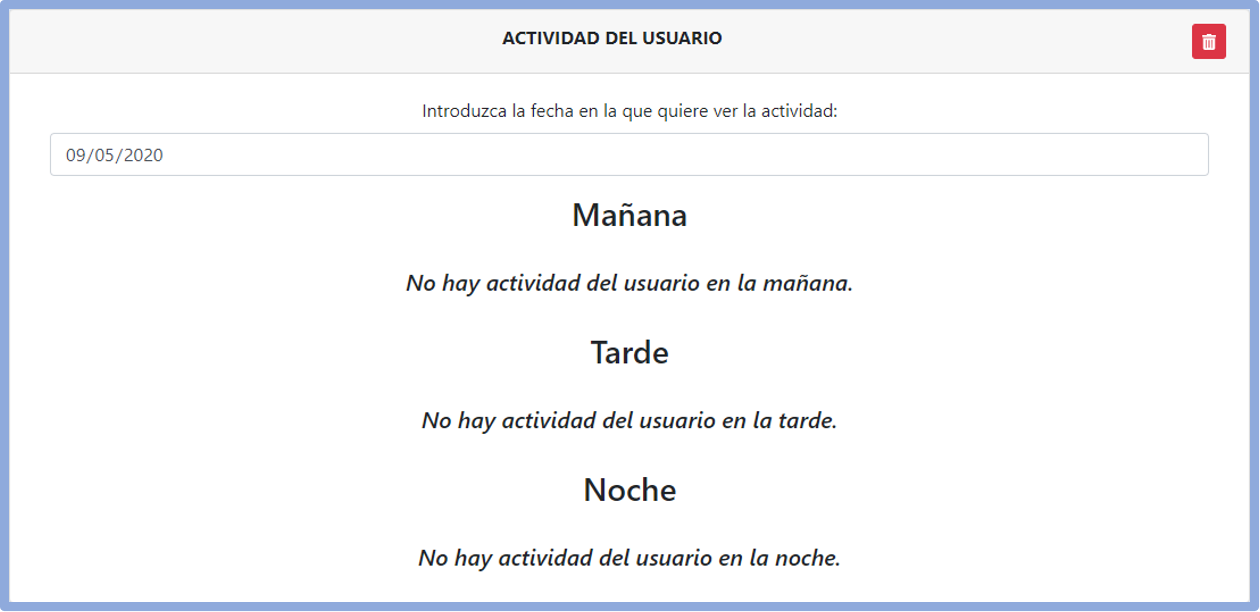
\includegraphics[width=.70\textwidth]{capitulos/capitulo10/actividad/1.png}
    \caption{Actividad antes de sacar el producto.}
    \label{fig:a1}
\end{figure}

\begin{figure}[h] 
    \centering
    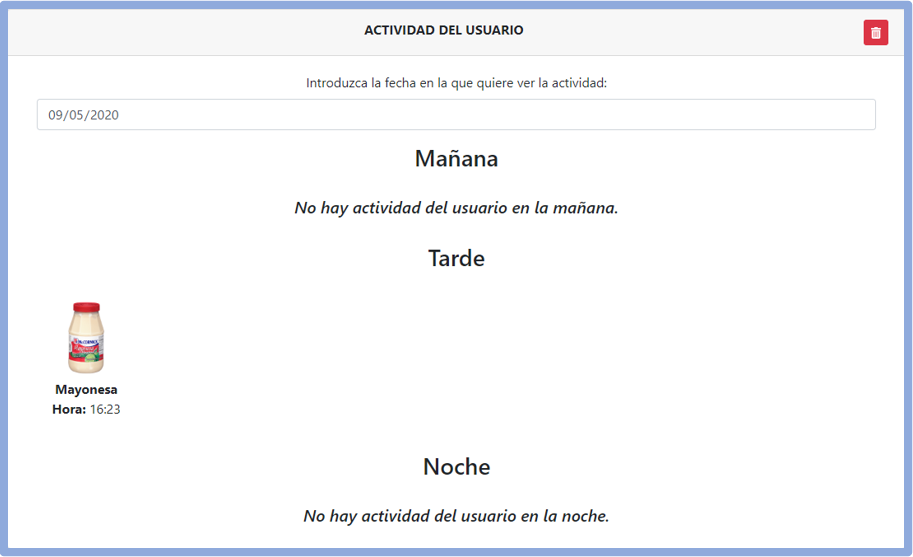
\includegraphics[width=.70\textwidth]{capitulos/capitulo10/actividad/2.png}
    \caption{Actividad después de sacar el producto.}
    \label{fig:a2}
\end{figure}

\newpage
Se puede ver está acción de forma más visual en un vídeo en el siguiente enlace: \url{https://youtu.be/UNocMCz9wYo}.

\section{Dieta}
El usuario puede especificar una dieta a seguir a lo largo de una semana. Se puede apreciar en al Figura \ref{fig:d1} como el usuario tiene que obtener un brik de leche por la mañana, y dos piezas de fruta por la tarde.

\begin{figure}[h] 
    \centering
    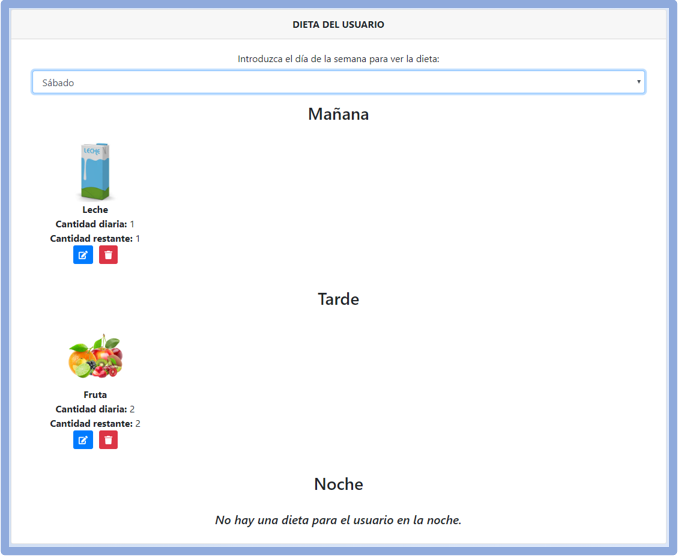
\includegraphics[width=.60\textwidth]{capitulos/capitulo10/dieta/1.png}
    \caption{Dieta estipulada para el usuario sin consumir.}
    \label{fig:d1}
\end{figure}

\newpage
Cuando se produce un cambio de parte del día, se envía un correo advirtiendo de los elementos a consumir en esa parte del día, otro correo si hay algún producto que no se ha consumido en la parte del día anterior. La simulación se hizo cuando la parte del día era la tarde, así que se envió un correo recordando que tenia que consumir dos piezas del fruta (Figura \ref{fig:d2}), y otro diciendo que no ha consumido el brik de leche que debería haber consumido por la mañana (Figura \ref{fig:d3}). Si hubiera consumido lo estipulado en al dieta por la mañana, éste último correo no se habría enviado.

\begin{figure}[h] 
    \centering
    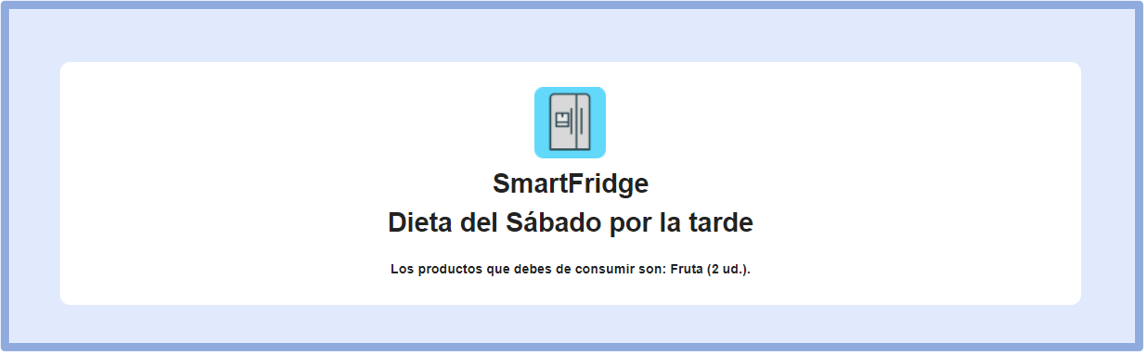
\includegraphics[width=.80\textwidth]{capitulos/capitulo10/dieta/2.png}
    \caption{Mensaje al usuario recordando que producto debe de consumir.}
    \label{fig:d2}
\end{figure}

\begin{figure}[h] 
    \centering
    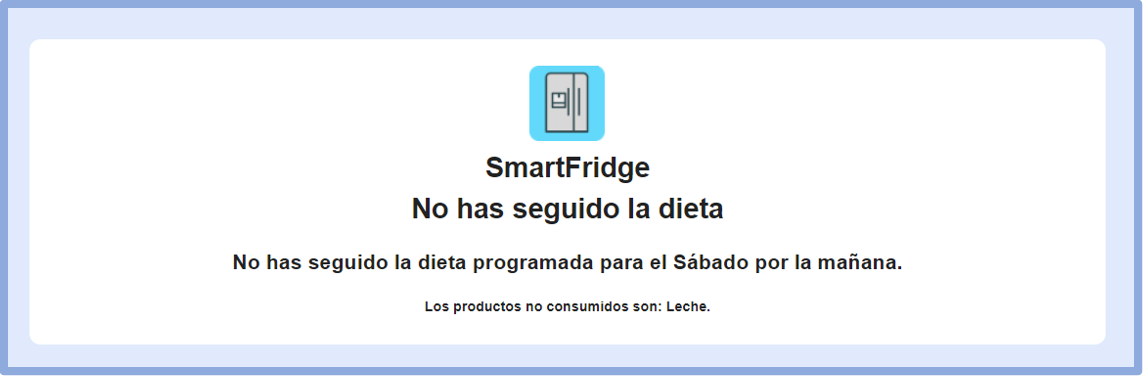
\includegraphics[width=.80\textwidth]{capitulos/capitulo10/dieta/3.png}
    \caption{Mensaje al usuario advirtiendo de productos de la dieta que no ha consumido.}
    \label{fig:d3}
\end{figure}

Finalmente, si el usuario sigue la dieta, en al interfaz se vería la dieta seguida, pero el parámetro de 'cantidad restante' estaría a cero, puesto que no falta nada por consumir (Figura \ref{fig:d4}).

\begin{figure}[!t] 
    \centering
    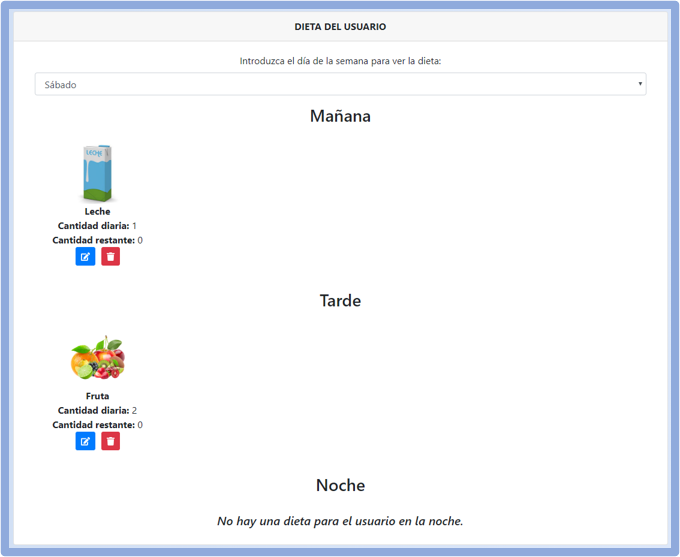
\includegraphics[width=.60\textwidth]{capitulos/capitulo10/dieta/4.png}
    \caption{Dieta estipulada para el usuario consumida.}
    \label{fig:d4}
\end{figure}

\newpage
Se puede ver está acción de forma más visual en un vídeo en el siguiente enlace: \url{https://youtu.be/fyPIuAnhHWs}.